%\documentclass[sigconf, authordraft]{acmart}
\documentclass[sigconf]{acmart}\usepackage[]{graphicx}\usepackage[]{color}
%% maxwidth is the original width if it is less than linewidth
%% otherwise use linewidth (to make sure the graphics do not exceed the margin)
\makeatletter
\def\maxwidth{ %
  \ifdim\Gin@nat@width>\linewidth
    \linewidth
  \else
    \Gin@nat@width
  \fi
}
\makeatother

\definecolor{fgcolor}{rgb}{0.345, 0.345, 0.345}
\newcommand{\hlnum}[1]{\textcolor[rgb]{0.686,0.059,0.569}{#1}}%
\newcommand{\hlstr}[1]{\textcolor[rgb]{0.192,0.494,0.8}{#1}}%
\newcommand{\hlcom}[1]{\textcolor[rgb]{0.678,0.584,0.686}{\textit{#1}}}%
\newcommand{\hlopt}[1]{\textcolor[rgb]{0,0,0}{#1}}%
\newcommand{\hlstd}[1]{\textcolor[rgb]{0.345,0.345,0.345}{#1}}%
\newcommand{\hlkwa}[1]{\textcolor[rgb]{0.161,0.373,0.58}{\textbf{#1}}}%
\newcommand{\hlkwb}[1]{\textcolor[rgb]{0.69,0.353,0.396}{#1}}%
\newcommand{\hlkwc}[1]{\textcolor[rgb]{0.333,0.667,0.333}{#1}}%
\newcommand{\hlkwd}[1]{\textcolor[rgb]{0.737,0.353,0.396}{\textbf{#1}}}%
\let\hlipl\hlkwb

\usepackage{framed}
\makeatletter
\newenvironment{kframe}{%
 \def\at@end@of@kframe{}%
 \ifinner\ifhmode%
  \def\at@end@of@kframe{\end{minipage}}%
  \begin{minipage}{\columnwidth}%
 \fi\fi%
 \def\FrameCommand##1{\hskip\@totalleftmargin \hskip-\fboxsep
 \colorbox{shadecolor}{##1}\hskip-\fboxsep
     % There is no \\@totalrightmargin, so:
     \hskip-\linewidth \hskip-\@totalleftmargin \hskip\columnwidth}%
 \MakeFramed {\advance\hsize-\width
   \@totalleftmargin\z@ \linewidth\hsize
   \@setminipage}}%
 {\par\unskip\endMakeFramed%
 \at@end@of@kframe}
\makeatother

\definecolor{shadecolor}{rgb}{.97, .97, .97}
\definecolor{messagecolor}{rgb}{0, 0, 0}
\definecolor{warningcolor}{rgb}{1, 0, 1}
\definecolor{errorcolor}{rgb}{1, 0, 0}
\newenvironment{knitrout}{}{} % an empty environment to be redefined in TeX

\usepackage{alltt}

\usepackage{booktabs} % For formal tables
\usepackage{tikz}
\usepackage{pgfbaselayers}
\usepackage[underline=false]{pgf-umlsd}
\usetikzlibrary{shadows}
\usetikzlibrary{arrows}

% Copyright
%\setcopyright{none}
%\setcopyright{acmcopyright}
%\setcopyright{acmlicensed}
\setcopyright{rightsretained}
%\setcopyright{usgov}
%\setcopyright{usgovmixed}
%\setcopyright{cagov}
%\setcopyright{cagovmixed}


% DOI
\acmDOI{10.1145/nnnnnnn.nnnnnnn}

% ISBN
\acmISBN{978-x-xxxx-xxxx-x/YY/MM}

% Conference
\acmConference[GECCO '19]{the Genetic and Evolutionary Computation Conference 2019}{July 13--17, 2019}{Prague, Czech Republic}
\acmYear{2019}
\copyrightyear{2019}

%\acmArticle{4}
\acmPrice{15.00}

% These commands are optional
%\acmBooktitle{Transactions of the ACM Woodstock conference}
%\editor{Jennifer B. Sartor}
%\editor{Theo D'Hondt}
%\editor{Wolfgang De Meuter}

\hypersetup{draft}
\IfFileExists{upquote.sty}{\usepackage{upquote}}{}
\begin{document}

\begin{knitrout}
\definecolor{shadecolor}{rgb}{0.969, 0.969, 0.969}\color{fgcolor}\begin{kframe}


{\ttfamily\noindent\itshape\color{messagecolor}{\#\# \\\#\# Attaching package: 'dplyr'}}

{\ttfamily\noindent\itshape\color{messagecolor}{\#\# The following objects are masked from 'package:stats':\\\#\# \\\#\#\ \ \ \  filter, lag}}

{\ttfamily\noindent\itshape\color{messagecolor}{\#\# The following objects are masked from 'package:base':\\\#\# \\\#\#\ \ \ \  intersect, setdiff, setequal, union}}\end{kframe}
\end{knitrout}

\title{Concurrency in evolutionary algorithms}

  \author{Anonymous Author 1}
  \orcid{1234-5678-9012}
  \affiliation{%
    \institution{Anonymous institute 1}
    \streetaddress{P.O. Box 1212}
    \city{Dublin}
    \state{Ohio}
    \postcode{43017-6221}
  }
  \email{aa1@ai1.com}
  
  \author{Anonymous Author 2}
  \affiliation{%
    \institution{Anonymous institute 2}
    \streetaddress{P.O. Box 1212}
    \city{Dublin}
    \state{Ohio}
    \postcode{43017-6221}
  }
  \email{2aa@ai2.com}

  \author{Anonymous Author 3}
  \affiliation{%
    \institution{Anonymous institute 2}
    \streetaddress{P.O. Box 1212}
    \city{Dublin}
    \state{Ohio}
    \postcode{43017-6221}
  }
  \email{2aa@ai2.com}

  \author{Anonymous Author 4}
  \affiliation{%
    \institution{Anonymous institute 2}
    \streetaddress{P.O. Box 1212}
    \city{Dublin}
    \state{Ohio}
    \postcode{43017-6221}
  }
  \email{2aa@ai2.com}
  
  % The default list of authors is too long for headers.
  \renewcommand{\shortauthors}{A. Author et al.}



\begin{abstract}
One of the core ideas behind the design of multi-threaded concurrent algorithms, is the concept of \emph{channel}, a computational device used to convey state to the different threads of processes that are executed concurrently. In the case of concurrent evolutionary algorithms, threads can be designed to perform different tasks within the evolutionary loop such as genetic operations or mixing of populations, and therefore they will need to communicate by passing messages across channels. In this paper we study to what extent the design of these messages in a communicating sequential processes context, may influence scaling and performance of concurrent evolutionary algorithms. For this aim, we designed a version of an algorithm and a communication model that is able to effectively solve different benchmark binary problems (e.g. OneMax, LeadingOnes, RoyalRoad), showing that it provides a good basis to leverage the multi-threaded and multi-core capabilities of modern computers. Although our results indicate that concurrency is advantageous to scale-up the performance of evolutionary algorithms, they also highlight how the trade--off between concurrency, communication and evolutionary parameters affect the outcome of the evolved solutions, opening-up new opportunities for algorithm design.

% One of the ways multi-threaded concurrent algorithms are designed 
% is around the concept of a channel, a structure
% used to convey state to the different threads that are running
% concurrently, which is why their design is one of the main challenges.
% Concurrent evolutionary algorithms will use threads, communicating via
% messages, for performing different types of tasks like evolving and
% mixing populations. In this paper we will explore the design of these
% messages in a communicating sequential processes context and with a 
% concurrent language and how it influences scaling and the performance of the
% algorithm itself. Eventually, we will show how a concurrent
% version of algorithms offer a good option to leverage the
% multi-threaded and multi-core capabilities of modern computers. In
% order to do this, we will explore the performance of the system by
% increasing the number of threads in order to find out the upper bounds
% for the speed up and the causes why they are reached. Results show
% that concurrency is achieved, but there the interaction between
% communication, the number of threads and the algorithm parameters is
% very important, opening new possibilities of algorithm design.

\end{abstract}

 \begin{CCSXML}
<ccs2012>
<concept>
<concept_id>10003752.10003809.10011778</concept_id>
<concept_desc>Theory of computation~Concurrent algorithms</concept_desc>
<concept_significance>500</concept_significance>
</concept>
<concept>
<concept_id>10010147.10010257.10010293.10011809.10011812</concept_id>
<concept_desc>Computing methodologies~Genetic algorithms</concept_desc>
<concept_significance>500</concept_significance>
</concept>
<concept>
<concept_id>10002944.10011123.10011674</concept_id>
<concept_desc>General and reference~Performance</concept_desc>
<concept_significance>300</concept_significance>
</concept>
</ccs2012>

\end{CCSXML}

\ccsdesc[500]{Theory of computation~Concurrent algorithms}
\ccsdesc[500]{Computing methodologies~Genetic algorithms}
\ccsdesc[300]{General and reference~Performance}

\keywords{Concurrency, Concurrent evolutionary algorithms, performance
evaluation, algorithm design}


\maketitle

\section{Introduction}

Despite the emphasis on leveraging newer hardware features
with best-suited software techniques
 there are not many papers \cite{Xia2010} dealing with 
creating concurrent evolutionary algorithms that work in a single
computing node or that extend seamlessly from single to many
computers. However, concurrent programming seems to be the best 
option if we are dealing with a multi-core processor architecture 
where many processes and threads can coexists at the same time. 
 This eventually means that many
processes (heavy or lightweight) can be leveraged to take full
advantage of the processor capabilities.

These capabilities must be matched at an abstract level by languages
that build on them so that high-level algorithms can use them without
worrying about the low-level mechanisms of creation or destruction of
threads, or how data is shared or communicated among them. These
languages are called concurrent, and the programming paradigm
implemented in them concurrency-oriented programming or simply
concurrent programming \cite{Armstrong2003}. 

These languages are characterized by the presence of
programming constructs that manage threads like first class
objects; that means that the language includes  operators for acting upon them and the
possibility of using them like parameters or function's result
values. This changes the coding of concurrent algorithms due to the
direct mapping between patterns of communications and processes with
% patterns of communication between processes? - Mario 
language expressions; on the one hand it becomes simpler since the
language provides an abstraction for communication, on the other hand
it changes the paradigm for implementing algorithms, since these new
communication constructs have to be taken into account. 

Moreover, concurrent programming adds a layer of abstraction over the parallel
facilities of processors and operating systems, offering a
high-level interface that allows the user to program modules of code to
be executed in parallel threads \cite{andrews1991concurrent}.

Different languages offer different concurrency strategies depending on how they deal with shared state,
that is, data structures that could be accessed from several processes or
threads. In this regard, there are two major fields and other, less well known models using, for instance, tuple
  spaces \cite{gelernter1985generative}:
\begin{itemize}
\item Actor-based concurrency \cite{schippers2009towards}
totally eliminates shared state by introducing a series of data
structures called {\em actors} that
store state and can mutate it locally. 
\item Process calculi or process algebra is a framework to describe
  systems that work with independent
  processes interacting between them using channels. One of the best
  known is called the {\em communicating sequential processes} (CSP)
methodology \cite{Hoare:1978:CSP:359576.359585}, which is effectively
stateless, with different processes reacting to a channel input without
changing state, and writing to these channels. Unlike actor based
concurrency, which keeps state local, in this case per-process state is totally
eliminated, with all computation state managed as messages in a channel.
\end{itemize}

Many modern languages, however, follow the CSP abstraction, and it has
become popular since it fits well other programming paradigms, like
reactive and functional programming, and allows for a more efficient
implementation, with less overhead, and with well-defined
primitives. This is why we will use it in this paper for creating  {\em natively}
concurrent evolutionary algorithms. We have chosen Perl 6, although 
other languages such as Go and Julia, are feasible alternatives.

In previous papers
\cite{Merelo:2018:MEA:3205651.3208317:anon,merelo:WEA:anon} we
designed an evolutionary algorithm that fits well this architecture
and explored its possibilities. That initial exploration showed that
a critical factor within this algorithmic model is the communication between threads; therefore designing
efficient messages is high-priority to obtain good algorithmic
performance and scaling. In this paper, we will test several
communication strategies: a loss-less one that compresses the population,
and a lossy one that sends a representation of gene-wise
statistics of the population.

\section{State of the Art}

The problem of communication/synchronization
between processes or threads, has been the subject of 
long-standing study, in order to to fully leverage multiple
processors and cores on a given machine. The parallelization of nature-based 
optimization algorithms has been an active field, allowing researchers
to solve complex optimization problems having a high computational 
cost \cite{Lalwani2019}. In the literature, most works are concerned 
with process-based concurrency, using for instance a Message Passing Interface 
(MPI) \cite{gropp1999using}, or hybrids with fine-grain
parallelization by using libraries such as OpenMP \cite{dagum1998openmp}
that offer multi-threading capabilities \cite{jin2011high}. Recent trends
in software development have motivated the inclusion of new 
constructs to programming languages with the intention of simplifying 
the development of multi-threaded programs. The theoretical support 
used by these implementations is based CSP. Languages such as Go 
and Perl 6 implement this concurrency model as an abstraction for 
their multi-threading capabilities. (the latter including additional mechanisms such as 
{\em promises} or low-level access to the creation of threads). Even 
interpreted languages with a global interpreter lock, such as Python also
have included {\em promises} and {\em futures} in their latest versions,
to leverage multi-threading capabilities for IO intensive tasks.
Using these native capabilities give developers the advantage of
having less error-prone implementations which are more readable and consistently
following the language conventions. 




% I think there could be confusion between the general "process" part 
% of an algorithm (from Process calculi), and an OS process (an instance of a program).a   
% So there is inter-process comunication/synchronization and
% inter-thread comunication/synchronization. For instance, Python can
% do a real parallel execution using processes and they can communicate 
% between them (RPC, RMI, Shared memory, message queues, etc.)
% Here, I think we are dealing only with communication between 
% threads. Python on the other hand cannot use two threads at the
% same time. - Mario


%One of the 
%best efforts to formalize and simplify that matter 
%is Hoare's {\em Communicating Sequential Processes} \cite{Hoare:1978:CSP:359576.359585},
%that proposes an interaction description language which is the 
%theoretical support for many libraries and modern programming 
%languages. In such model, concurrent programs communicate on 
%the basis of {\em channels}, a sort of pipe buffer used to
%interchange messages between the different processes or threads, 
%either asynchronously or synchronously. 

The fact that messages have to be processed without secondary effects
and that actors do not share any kind of state makes concurrent
programming specially fit for functional languages or languages with
functional features; this has made this paradigm specially popular for
late cloud computing implementations; however, its presence in the EA
world is not so widespread, although some efforts have lately revived
the interest for this kind of paradigm \cite{swan2015research}.
Several years ago it was used in Genetic Programming
\cite{Briggs:2008:FGP:1375341.1375345,Huelsbergen:1996:TSE:1595536.1595579,walsh:1999:AFSFESIHLP}
and recently in neuroevolution \cite{Sher2013} but its occurrence in EA,
despite being scarce in the previous years
\cite{Hawkins:2001:GFG:872017.872197}, has experimented a certain rise
lately with papers such as \cite{valkov2018synthesis} which perform
program synthesis using the functional programming features of the Erlang language
\cite{barwell2017using} for building an evolutionary multi-agent system.

Regarding functional languages, Erlang and Scala have
embraced the actor model of concurrency and get excellent results in
many application domains; Clojure is another one with concurrent
features such as promises/futures, software transactional memory (STM) 
and agents; Kotlin \cite{simson2017open} has been recently used for
implementing a functional evolutionary algorithm framework.  

On the
other hand, Perl 6 \cite{Tang:2007:PRI:1190216.1190218,lenzperl} 
uses different concurrency models, varying from implicit concurrency 
using the {\tt hyper} and {\tt race} functions, that automatically 
parallelize operations on iterable data structures, to explicit 
concurrency using threads. 
The {\tt Algorithm::Evolutionary::Simple} library introduced last year
%\cite{DBLP:conf/gecco/GuervosV18}
.

Earlier efforts to study the issues of concurrency in EA are worth 
mentioning. For instance, the EvAg model \cite{evag:gpem} resorts to 
the underlying platform scheduler to manage the different threads of 
execution of the evolving agents; in this way the model scaled-up 
seamlessly to take full advantage of CPU cores. In the same avenue 
of measuring scalability,  experiments were conducted
in \cite{wcci:evoag} comparing single and a dual-core processor 
concurrency achieving near linear speed-ups . The latter
was later on extended in \cite{DBLP:conf/evoW/LaredoBMG12} by scaling
up the experiment to up to 188 parallel machines, reporting speed-ups 
up to $960\times$, nearly four times the expected linear growth 
in the number of machines (when local concurrency were not taken 
into account). Other authors have addressed explicitly multi-core 
architectures, such as Tagawa \cite{Tagawa201212} which used 
shared memory and a clever mechanism to avoid deadlocks. Similarly,
\cite{kerdprasop2012concurrent} used a message-based architecture 
developed in Erlang, separating GA populations as different
processes, although all communication was taking place with a common
central thread. 


In previous papers 
\cite{Merelo:2018:MEA:3205651.3208317:anon,Garcia-Valdez:2018:MEA:3205651.3205719:anon},
we presented a proof of concept of the implementation of a stateless 
evolutionary algorithms using Perl 6, based on a single 
channel model communicating threads for population evolving and 
mixing. In addition, we studied the effect of running parameters 
such as the {\em generation gap} (similar to the concept of {\em
time to migration} in parallel evolutionary algorithms) and 
population size, realizing that the choice of parameters may have 
a strong influence at the algorithmic level, but also at the 
implementation level, in fact affecting the actual wallclock
performance of the EA.

\section{Setting up the experiments using an evolutionary algorithm library in Perl 6}

Perl 6 is a concurrent, functional language
\cite{DBLP:journals/corr/abs-1809-01427} which was conceived with the
intention of providing a solid conceptual framework for multi-paradigm
computing, including thread-based concurrency and asynchrony. It's got
a heuristic optimization model, which literally optimizes code as it
runs. Its speed has been improving by a factor of 100x in the last few
years, with a performance that is in the same scale than interpreted
languages, although with some room for improvement.

The {\tt Algorithm::Evolutionary::Simple} Perl 6 module was published
in the ecosystem a year ago, and got recently into version 0.0.7. It
is a straightforward implementation of a canonical evolutionary
algorithm with binary representation, and includes building blocks for
a generational genetic algorithm, as well as some fitness functions
used generally as benchmarks.

Those evolutionary algorithm building blocks do not include concurrent
primitives; it's up to the developer to design a concurrent
evolutionary algorithm using it.

\begin{figure}[h!tb]
  \centering
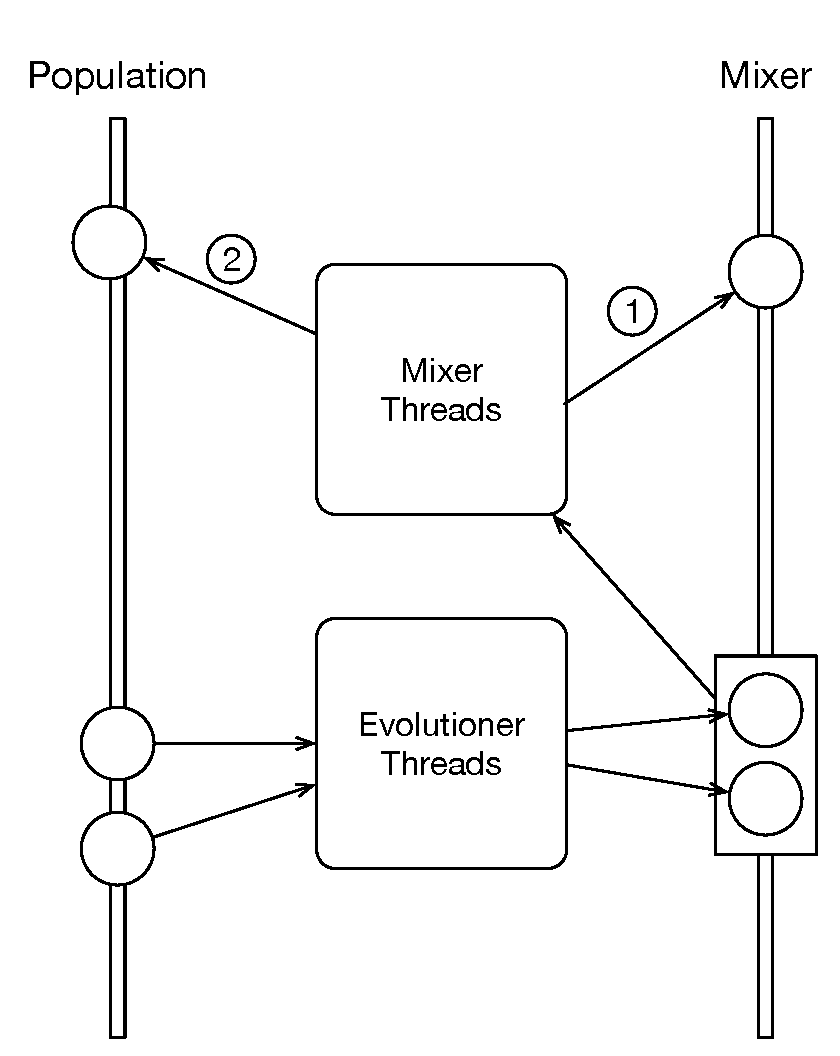
\includegraphics[width=0.95\columnwidth]{../figure/popmixer}
\caption{General scheme of operation of channels and thread groups. }
\label{fig:scheme}
\end{figure}
%

\begin{figure}[h!tb]
  \centering
  
\begin{sequencediagram}

\newthread[red]{E}{Evolver} 

\tikzstyle{inststyle}+=[rounded corners=3mm] 
\newinst{C}{Channel}

\tikzstyle{inststyle}+=[rounded corners=0]
\newthread[blue]{M}{Mixer}

\begin{call}{E}{evolve()}{E}{}\end{call}

\setthreadbias{east}
\begin{messcall}{E}{$pop_1$}{C} 
\mess{C}{$pop_1$}{M}
\end{messcall}

\prelevel\prelevel
\begin{call}{E}{evolve()}{E}{}\end{call}

\setthreadbias{east}
\begin{messcall}{E}{$pop_2$}{C}  
\mess{C}{$pop_2$}{M}
\end{messcall}

\prelevel\prelevel
\begin{call}{M}{mix()}{M}{}\end{call}

\postlevel\postlevel
\setthreadbias{west}
\begin{messcall}{M}{\shortstack{ \{\ $mixpop_1$,\\ $mixpop_2$,\\ \vdots \\ $mixpop_k$ \} }}{C}

\mess{C}{$mixpop_1$}{E} 
\begin{call}{E}{evolve()}{E}{}\end{call}

\setthreadbias{east}
\begin{messcall}{E}{$pop_3$}{C} 
\postlevel
\mess{C}{$mixpop_2$}{E} 
%\prelevel
\mess{C}{$pop_3$}{M}
\end{messcall}

\prelevel\prelevel
\begin{call}{E}{evolve()}{E}{}\end{call}

\setthreadbias{east}
\begin{messcall}{E}{$pop_4$}{C}
\mess{C}{$pop_4$}{M}
\end{messcall}

\setthreadbias{west}
\prelevel
\mess{C}{$mixpop_k$}{E}%\end{messcall}

\end{messcall}

\prelevel\prelevel
\begin{call}{M}{mix()}{M}{\vdots}\end{call}
\prelevel
\begin{call}{E}{evolve()}{E}{\vdots}\end{call}

\end{sequencediagram}

\caption{Schematic of communication between threads and channels for
  concurrent EAs. The two central bars represent the channel, and
  color corresponds to the {\em main} function they perform; blue for
  mixer, red for evolver. As the figure shows, the evolver threads
  always read from the mixer channel, and always write to the evolver
  channel.}
\label{fig:schematic}
\end{figure}


The baseline we are coming from is similar to the one used in previous experiments
\cite{Merelo:2018:MEA:3205651.3208317:anon}. Our intention was to
create a system that was not functionally equivalent to a sequential
evolutionary algorithms, and that followed the principle of
communicating sequential processes. In this kind of methodology, we
will have processes (or threads) communicating state through
channels. Every process itself will be stateless, reacting to the
presence of messages in the channels it is listening to and sending
result back to them, without changing state.

As in the previous papers, \cite{merelo:WEA:anon}, we will use two
groups of threads and two channels. We will see them in turns.

The two groups of threads perform the following
functions:\begin{itemize}
\item The {\em evolutionary} threads will be the ones that will be in
  principle running the evolutionary algorithm.
\item The {\em mixing} thread will {\em mix} populations, and create
  new ones as a mixture of them.
\end{itemize}

The two channels carry messages that are equivalent to populations,
but they do so in a different way:\begin{itemize}
  
\item The {\em evolutionary} channel will be used for carrying
  non-evolved, or generated, populations.
\item The {\em mixer} channel will carry, {\em in pairs}, evolved
  populations. 
\end{itemize}

These will be connected as shown in Figure \ref{fig:scheme}. The
evolutionary thread group will read only from the evolutionary channel,
evolve for a number of generations, and place result in the mixer
channel; the mixer group of threads will read only from the mixer
channel, in pairs. From every pair, a random element is put back into
the mixer channel, and a new population is generated and sent back to
the evolutionary channel. The main objective of using two channels is
to avoid deadlocks; the fact that one population is written always
back to the mixer channel avoids starvation in the channel. How this
runs in practice is shown in Figure \ref{fig:schematic}, where the
timeline of the interchange of messages between the evolver and mixer
threads and evolver and mixer channels is clarified.

The state of the algorithm will be transmitted via messages that
contain data about one population. Since using the whole population
will incur in a lob of overhead, we use a strategy that is similar to {\em EDA}, or estimation of distribution
  algorithm, whose basic idea is that the population message will
  contain the probability distribution over each gene. In this sense,
  this strategy is similar to the one presented by de la Ossa et
  al. in \cite{10.1007/978-3-540-30217-9_25}. Not being an estimation
  of distribution algorithm {\em per se}, since the evolutionary
  thread runs a canonical genetic algorithm, when the message is being
  composed, every (binary) gene of the 25\% best individuals in the
  population is examined, and an array with the
  probabilities for each gene is sent to the mixer thread. The {\em
    mixer} thread, in turn, just takes randomly one probability from
  each of the two {\em populations} (actually, distributions), instead
  of working on individuals. While in the baseline strategy the
  selection took place in the mixer thread, that eliminated half the
  population, in this case the selection takes place when composing
  the message, since just the 25\% best individuals are selected to
  compute the probability distribution of genes. When the evolver
  thread reads the message, it rebuilds the population based on this
  distribution.

\section{Experimental results}
\label{sec:exp}

We were mainly interested in the scaling capabilities of the algorithm
and implementation, so we tested several benchmark, binary functions:
OneMax, Royal Road and Leading Ones, all of them with 64 bits. 




\begin{figure*}[h!tb]
  \centering
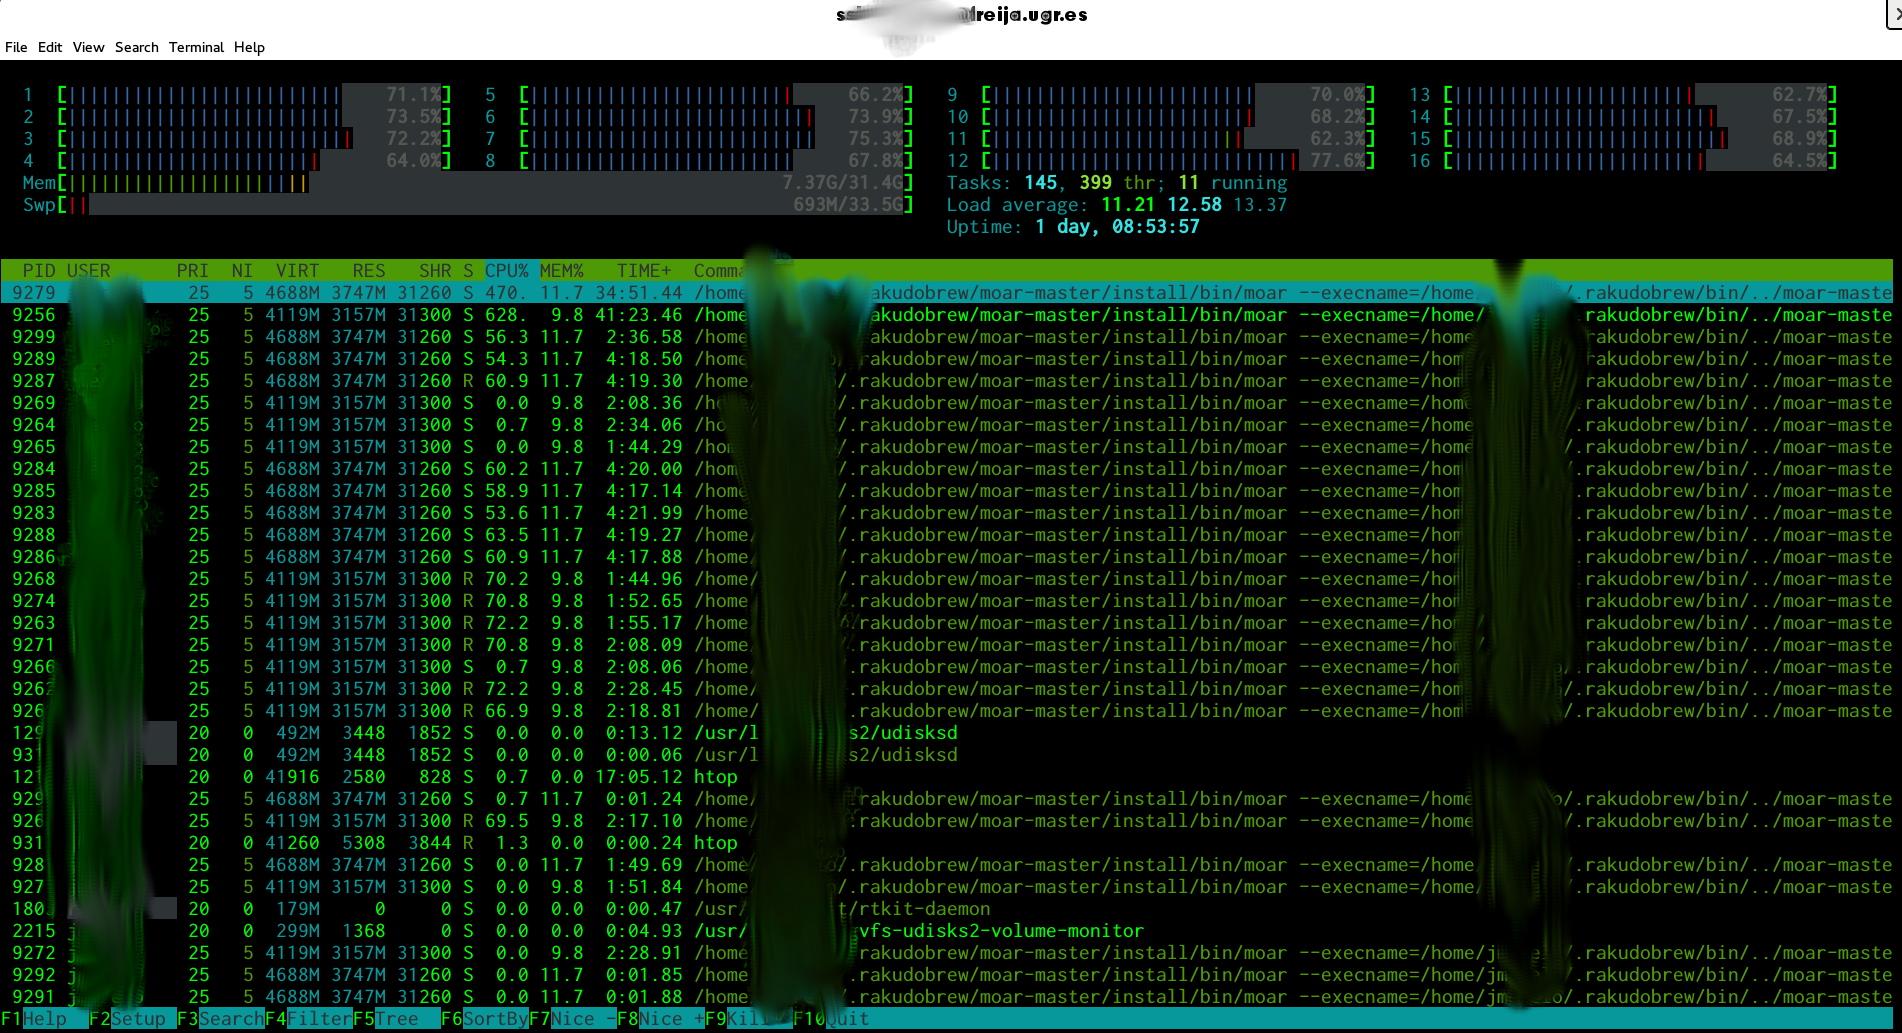
\includegraphics[width=0.95\textwidth]{../figure/screenshot}
\caption{Screenshot using the htop utility of the used machine running
  two experiments at the same time. As it can be seen, all processors
  are kept busy, with a very high load average. }
\label{fig:screenshot}
\end{figure*}
%
However, the intention of concurrent evolutionary algorithms is to
leverage the power of all threads and processors in a computer so we must find out how it scales for different fitness functions. We are setting the number of initial populations was set to the
number of threads plus one, as the minimum required to avoid
starvation, and we are using a single mixing thread. As proved in our previous paper (hidden for anonymity), we are dividing the total population by the number of threads. The initial population will be 1024 for OneMax, 8192 for Royal Road and 4096 Leading Ones. These quantities were found heuristically by applying the bisection method on a selectorrecombinative algorithm, which doubles the population until one that is able to find the solution 95\% of the time is found.

Experiments were run on a machine with the
Ubuntu 18.04 OS and an AMD Ryzen 7 2700X Eight-Core Processor
at 3.7GHz, which theoretically has 8 x 16 = 128 physical
threads. Figure \ref{fig:screenshot} shows the utility  {\tt htop} with an 
experiment running; the top of the screen shows the rate at which all
cores are working, showing all of them occupied; of course, the
program was not running exclusively, but the list of processes below
show how the program is replicated in several processor, thus
leveraging their full power. Please check also the number of threads
that are actually running at the same time, a few of which are being used by our application; these are not, however, physical but operating system threads; the OS is able to accommodate many more threads that are physically available if the code using them is idle. 

\begin{figure}[h!tb]
  \centering
\begin{knitrout}
\definecolor{shadecolor}{rgb}{0.969, 0.969, 0.969}\color{fgcolor}
\includegraphics[width=\maxwidth]{figure/threads1-1} 

\end{knitrout}
\caption{OneMax: Number of evaluations vs. number of threads. Higher is better.}
\label{fig:threads1}
\end{figure}
%
\begin{figure}[h!tb]
  \centering
\begin{knitrout}
\definecolor{shadecolor}{rgb}{0.969, 0.969, 0.969}\color{fgcolor}
\includegraphics[width=\maxwidth]{figure/threads2-1} 

\end{knitrout}
\caption{OneMax: Total time vs. number of threads. Lower is better.}
\label{fig:threads2}
\end{figure}
%
We are first interested in the number of evaluations needed to find
the solution, which are plotted in Fig. \ref{fig:threads1}, since, as
indicated from the beginning, there is going to be an interaction
between the performance of the algorithm and the way it is
implemented, spreading it over different threads. In this case, and
looking at the similarity with island-based parallel EAs, population
does have an influence on the number of evaluations, with bigger
populations tipping the balance in favor of exploration and thus
making more evaluations to achieve the same result; the same happens
with smaller populations, they tend to reach local minima and thus
also increase exploration. Figure \ref{fig:threads1} shows how the
overall number of populations
increases slightly and not significantly from 2 to 4 threads, but it
does increase significantly for 6 and 8 threads, indicating that the
algorithm's performance is worse when we increase the number
of threads, and consequently we need more evaluations to achieve the
same result. This is probably due to the fact that we are
simultaneously decreasing the population size, leading to earlier
convergence for the number of generations (8) it is being used. This
interplay between the degree of concurrency, the population size and
the number of generations will have to be explored further.

\begin{figure}[h!tb]
  \centering
\begin{knitrout}
\definecolor{shadecolor}{rgb}{0.969, 0.969, 0.969}\color{fgcolor}
\includegraphics[width=\maxwidth]{figure/threads3-1} 

\end{knitrout}
\caption{OneMax: Evaluations per second vs. number of threads. Higher is better.}
\label{fig:threads3}
\end{figure}
%
But we were also interested in the actual wallclock time, plotted in
Fig. \ref{fig:threads2}. The picture shows that it decreases
significantly when we go from 2 (the baseline) to 4 threads, since we
are using more computing power for (roughly) the same number of
evaluations. It then increases slightly we we increase the number of
threads; as a matter of fact and as shown in \ref{fig:threads3}, the
number of evaluations per second increases steeply up to 6 threads,
and slightly when we use 8 threads. However, the amount of evaluations
needed overcompensates this speed, resulting in a worse results. It
confirms, however, that we are actually using all threads for
evaluations, and if only we could find a strategy that didn't need
more evaluations we should be able to get a big boost in computation
time that scales gracefully to a high number of processors.

\begin{figure}[h!tb]
  \centering
\begin{knitrout}
\definecolor{shadecolor}{rgb}{0.969, 0.969, 0.969}\color{fgcolor}
\includegraphics[width=\maxwidth]{figure/threads-rr1-1} 

\end{knitrout}
\caption{Royal Road: Number of evaluations vs. number of threads. Higher is better.}
\label{fig:threads:rr:1}
\end{figure}
%
\begin{figure}[h!tb]
  \centering
\begin{knitrout}
\definecolor{shadecolor}{rgb}{0.969, 0.969, 0.969}\color{fgcolor}
\includegraphics[width=\maxwidth]{figure/threads-rr2-1} 

\end{knitrout}
\caption{Royal Road: Total time vs. number of threads. Lower is better.}
\label{fig:threads:rr:2}
\end{figure}
%
\begin{figure}[h!tb]
  \centering
\begin{knitrout}
\definecolor{shadecolor}{rgb}{0.969, 0.969, 0.969}\color{fgcolor}
\includegraphics[width=\maxwidth]{figure/threads-rr3-1} 

\end{knitrout}
\caption{Royal Road: Evaluations per second vs. number of threads. Higher is better.}
\label{fig:threads:rr:3}
\end{figure}

But we were interested also in checking whether the same kind of
patterns are found for other fitness functions, with a different
landscape, and also how much further scaling with the number of
threads could go; that is why we set up another experiment with the
Royal Road function. The next figures starting with \ref{fig:threads:rr:1} chart the results obtained for it. We run the experiment as above, but in this case there were
some runs in which the solution was not found within the time limit of
800 seconds; in the first case, for two threads, this is indicated
with a lighter shade corresponding to the number of instances where it
did found the solution, 6 out of 15. The number of evaluations needed
to find the solution is shown as a boxplot in Figure
\ref{fig:threads:rr:1}; the total time in Figure
\ref{fig:threads:rr:2} and the number of evaluations per second in
Figure \ref{fig:threads:rr:3}. Since the Royal Road function is
slightly heavier than onemax, this number reaches a peak that is
approximately 25\% lower than for onemax. Comparing also Figures
\ref{threads1} with \ref{fig:threads:rr:2} we see that that Royal Road
needs one order of magnitude more evaluations than OneMax to find the
solution. Since we cap the running time at 800 seconds, this causes
the lack of success in some cases for the lowest number of threads.

The pattern these charts follow is very similar to the one for
OneMax. The performance scales up to a certain range, and then it
plateaus, scaling only in speed, but not in wallclock time. From 2 to
6 threads speed increases 2x, due to an increase in speed with a
slight decrease in the number of evaluations needed to find the
solution; besides, success rate goes up from 2 to 4 threads, going
from finding the solution 6 out of 15 times to finding it every
time. This is basically due to the cap in the time allowed to run,
which is 800 seconds; it is likely that if more time had been allowed,
solution had been found. However, the fact is that we again find the
same effect of increase in performance, up to an optimal number of
threads, which is 6 in this case. This is slightly better than it was
for onemax, which reached an optimal performance for 4 threads. The
fact that the optimal population in Royal Road is 4x that needed for
OneMax will probably have an influence in that fact; as a rule of
thumb, performance will only increase to the point that population
size will make the algorithm worsen in the opposite
direction. However, it also proves that the peak performance is mainly
due to algorithmic, not the physical number of threads (which should
be around 16 for this machine). Finding an algorithmic solution to
this problem would allow us to leverage the number of threads
available in a machine even more.

\section{Conclusions}
\label{sec:conclusions}

Designing a concurrent, stateless evolutionary algorithm brings a new
set of configuration decisions that must be taken into account at the algorithm and
at the parameter level. In previous papers we have established
strategies that have allowed us to take advantage of processor threads
to achieve better wallclock performance through the design of messages
and channels to interchange between threads and a procedure to divide
the population between them. In this paper we wanted to focus on the
software tool that we have used for performing these experiments, as
well as to check what kind of scaling we can achieve on different
types of problems. 


What we have observed is that, since OneMax is a simple problem which
needs a small population to find the solution, scaling is very limited
and only means a real improvement if we use four threads instead of
two, getting no further improvement. That is why we experimented with
the Royal Road function with the same length, which showed an
interesting behavior in the sense that it scaled in success rate and
speed from 2 to 4 threads, and then again in speed through 6
threads. In this experiment we measured up to 12 threads, and we
noticed that the number of evaluations per second also reaches a
plateau at around 6k evaluations. For 8 threads, our program uses
actually 9 threads since there is another one for mixing. Since the
computer only has 16 physical threads (2 threads x 8 cores), and
taking into account other system programs, this is probably due to a
physical limit. Anyway, peak performance is reached for 6 processors,
so we need to reconsider the problem again in order to be able to
reach this limit.


Although the good performance of this concurrent evolutionary
algorithm has been well established in this paper, several lines of
research are open. The first one is to continue exploring the
algorithm itself trying to find out a scaling strategy that does not
have a negative influence in the number of evaluations, so that actual
increasing in the number of simultaneous evaluations achieved the
equivalent speedup. The second one would be to find out what is the
maximum number of simultaneous evaluations that can be achieved, so
that an optimum number of threads can be advised, if possible
independently of the problem and depending only on the physical number
of cores available.

The messaging strategies proposed here can be used only if the problem
can be represented via a binary data structure. New strategies will
have to be explored for floating-point representation, or more
complicated data structures. There are general-purpose strategies for
compressing messages, for instance, and they could be used in this
case. Estimation of distribution algorithms can also be extended to
other types of data, so this is is something that can be also explored.

Finally, we are using the same kind of algorithm in all
threads. Nothing prevents us from using a different algorithm per
thread, or using different parameters per thread. This opens a vast
space of possibilities, but the payoff might be worth it.



\begin{acks}
Acknowledgements taking\\
this much\\
space

\end{acks}

\bibliographystyle{ACM-Reference-Format}
\bibliography{../geneura,../concurrent,../perl6} 

\end{document}
